% 第 14 题翻折图：按固定源 PDF 矢量路径换算（1 pt → 0.03515 cm）。
% 原点取 C 点（源页 (565.39, 736.24) pt），y 向上。
% 平面四边形 ABCD：AC 为翻折轴（实线）；D 到 A、C 两边为虚线（翻折前位置）；
% 翻折后 D′ 到 A、C 两边为实线；BA、BC 实线。虚实归属由各路径 stroke-dasharray 直接判定。
% 各顶点旁标注 A/B/C/D/D′（照源字形框中心）。源图为示意（不按比例），照源复刻。
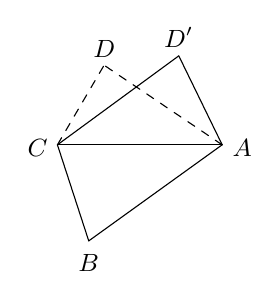
\begin{tikzpicture}[line cap=round,line join=round,font=\small,x=0.03515cm,y=0.03515cm]
\draw (59.51,0)--(0,0);                % A–C（翻折轴）
\draw (11.31,-34.71)--(0,0);           % B–C
\draw (11.31,-34.71)--(59.51,0);       % B–A
\draw (0,0)--(43.84,32.14);            % C–D′
\draw (59.51,0)--(43.84,32.14);        % A–D′
\draw[dash pattern=on 2.99pt off 2.99pt] (0,0)--(16.86,28.76);      % C–D（虚线，翻折前位置）
\draw[dash pattern=on 2.99pt off 2.99pt] (59.51,0)--(16.86,28.76);  % A–D（虚线，翻折前位置）
% ===== 标签（照源字形框中心，显式坐标）=====
\node[anchor=center,inner sep=0] at (66.72,-1.14) {\(A\)};
\node[anchor=center,inner sep=0] at (11.27,-42.84) {\(B\)};
\node[anchor=center,inner sep=0] at (-7.13,-1.14) {\(C\)};
\node[anchor=center,inner sep=0] at (16.94,34.61) {\(D\)};
\node[anchor=center,inner sep=0] at (43.82,38.74) {\(D'\)};
\end{tikzpicture}
